\label{sec:models}\vspace{-3mm}


\begin{figure}[t]
\begin{center}
\subfigure[]{
\raisebox{1mm}{
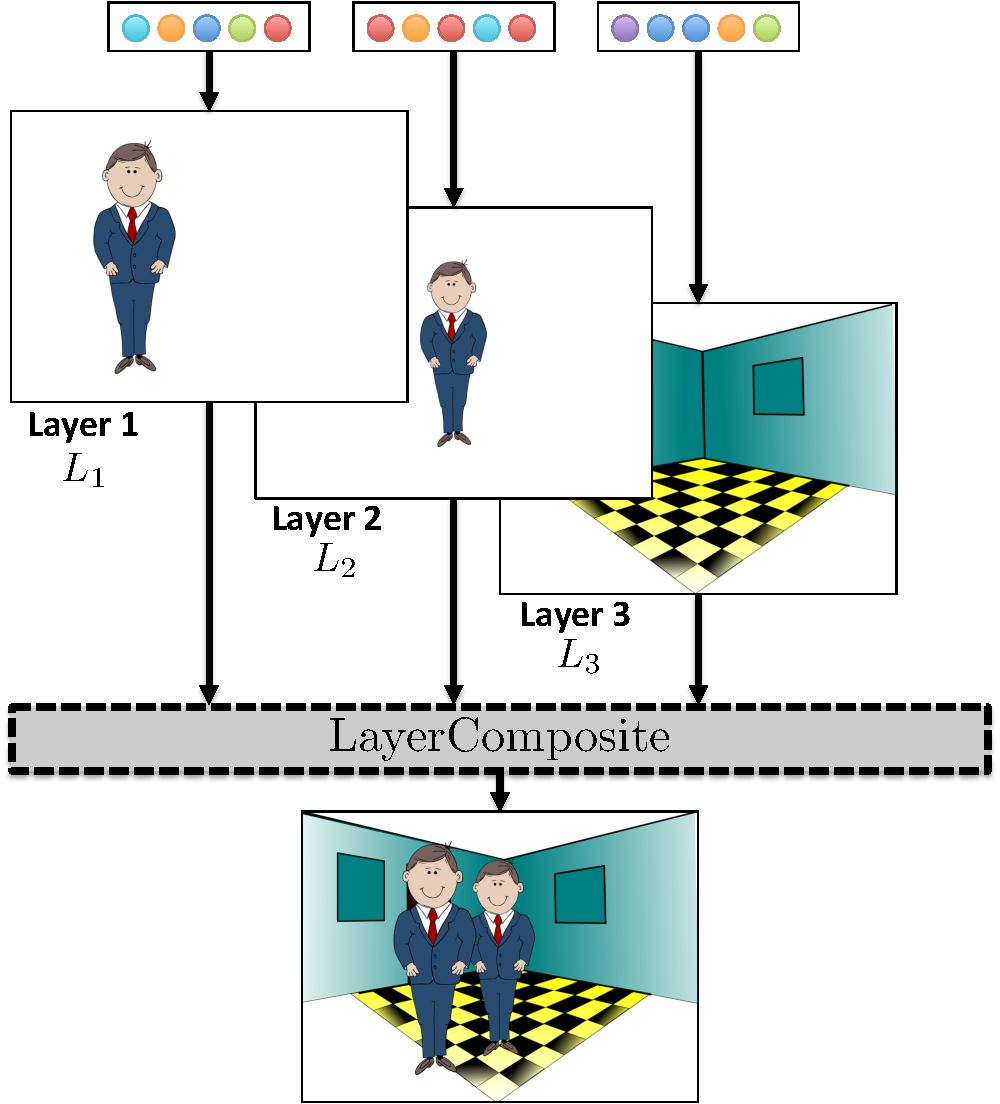
\includegraphics[width=0.30\linewidth]{figs/cartoon.pdf}
\label{fig:cartoon}
}
}\qquad\qquad\qquad
\subfigure[]{
%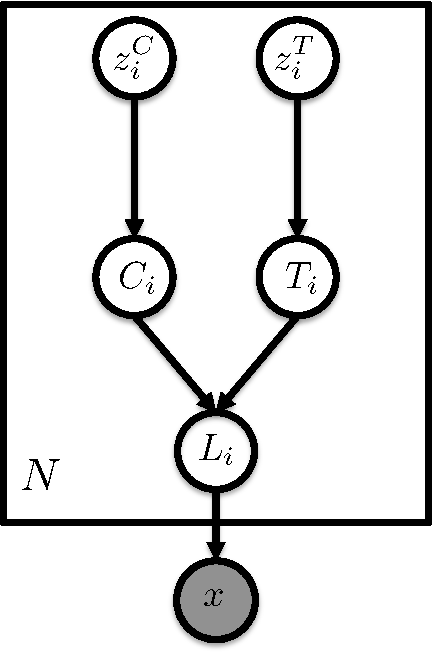
\includegraphics[width=0.2\linewidth]{figs/compositestvae_graphicalmodel.pdf}
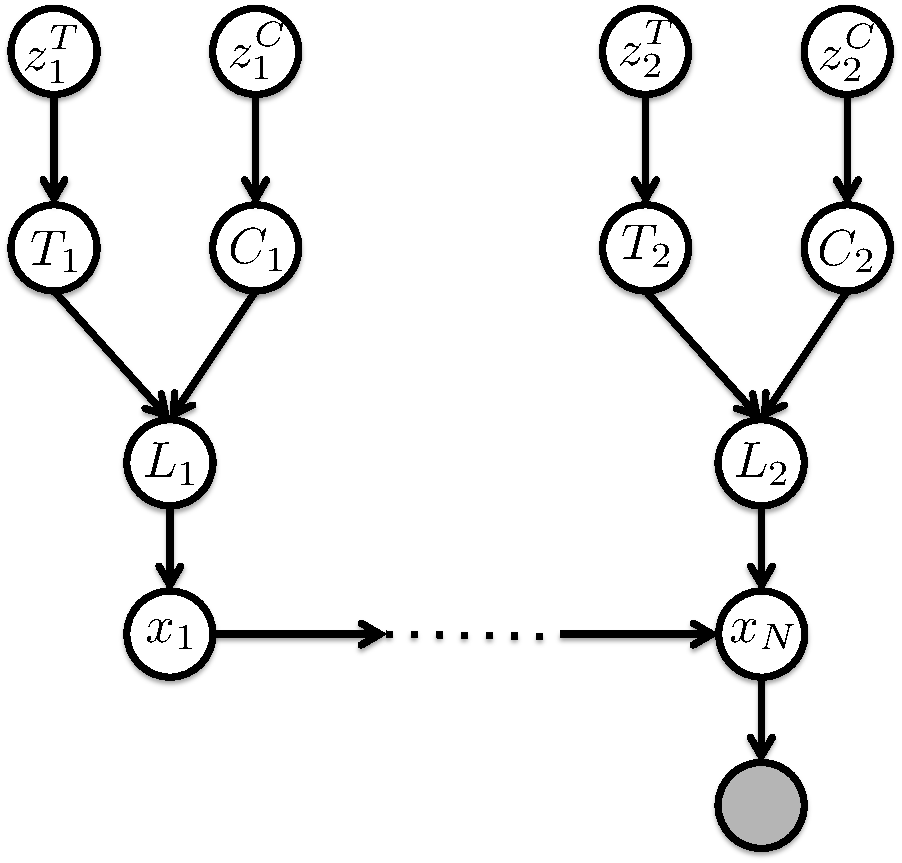
\includegraphics[width=0.35\linewidth]{figs/cstVae2.pdf}
\label{fig:compositestvae_gm}
}\vspace{-5mm}
\end{center}
 \caption{\footnotesize \subref{fig:cartoon} Cartoon illustration of the CST-VAE layer compositing process; 
 \subref{fig:compositestvae_gm} CST-VAE graphical model.  
%The boxed  portion of the graph (plate notation) is duplicated $N$ times. 
%\Jon{fix notation here and label the cartoon with variables}.
% Note that the order of the layers matters (to reflect that foreground can occlude background but not vice versa).
 }\vspace{-3mm}
\end{figure}


In this section we introduce the \emph{Composited Spatially Transformed Variational Auto-encoder  (CST-VAE)},
a family of latent variable models, which factors
the appearance of an image into the appearance of the different layers
that create that image.  
Among other things, the CST-VAE model allows us to tease
apart the component layers (or objects) that make up an image and
reason about occlusion in order to perform tasks such as amodal
completion 
\citep{Kar2015}
or instance segmentation
\citep{Hariharan2014}.
Furthermore, it can be trained in a fully unsupervised fashion using  minibatch stochastic
gradient descent methods but can also make use of labels in supervised or semi-supervised settings.
 
 In the CST-VAE model, we assume that images are created by (1) generating a sequence of image layers,
 then (2) compositing the layers to form a final result.  Figure~\ref{fig:cartoon} shows a simplified cartoon illustration of this process.  
 We now discuss these two steps individually.
 \vspace{-1mm}
 \paragraph{Layer generation via the ST-VAE model.}
 The layer generation model is interesting in its own right and we will call it the \emph{Spatially transformed 
 Variational Auto-Encoder (ST-VAE) model} (since there is no compositing step).
 We intuitively think of  layers as corresponding to objects in a scene --- a layer $L$ is assumed 
 to be generated by first generating an image $C$ of an object in some canonical pose (we refer to this image as
 the \emph{canonical image} for layer $L$), then warping $C$ in the 2d image plane (via some transformation $T$).
We assume that both $C$ and $T$ are generated by some latent variable --- specifically $C = f_C(z^C; \theta_C)$ and $T = f_T(z^T; \theta_T)$,
where $z^C$ and $z^T$ are latent variables and $f_C(\cdot; \theta_C)$ and $f_T(\cdot; \theta_T)$ are nonlinear functions with parameters
$\theta_C$ and $\theta_T$ to be learned.  We will call these content
and pose generators/decoders.
We are agnostic as to the particular parameterizations of $f_C$ and $f_T$, though as we discuss below, they
are assumed to be almost-everywhere differentiable and in practice we
have used MLPs.
% and convolutional networks.
In the interest of seeking simple interpretations of images, we also assume that these latent pose and content ($z^C$, $z^T$) 
variables are low-dimensional and independently Gaussian.

Finally to obtain the warped image, we
use \emph{Spatial Transformer Network} (STN) modules, recently introduced by~\cite{jaderberg2015spatial}.
We will denote  the result of resampling an image $C$ onto a regular grid which has been transformed by $T$ by $STN(C, T)$.
The benefit of using STN modules in our setting 
is that they perform resampling in a differentiable way, allowing for our models to be trained using gradient methods.
 \vspace{-1mm}
\paragraph{Compositing.}
To form the final observed image of the (general multi-layer) CST-VAE model, we generate a sequence of layers $L_1$, $L_2$, \dots, $L_N$
independently drawn from the ST-VAE model and composite from
front to back.
%back to front.
There are many  ways to composite multiple layers in computer graphics~\citep{porter1984compositing}.
In our experiments, we use  the classic \emph{over operator}, which reduces to a simple $\alpha$-weighted
convex combination of foreground and background pixels (denoted as a  binary  operation $\oplus$)
in the two-layer setting, but can be iteratively applied
to handle multiple layers. % associativity of the over operator

 

To summarize, the CST-VAE model can be written as the following generative process.  Let $x_0=\mathbf{0}^{w\times h}$ (i.e., a black image).   For $i=1,\dots,N$:\vspace{-4mm}

{\footnotesize
\begin{align*}
z_i^C, z_i^T  &\sim \mathcal{N}(0, I), \\
C_i &= f_C(z_i^C; \theta_C), \\
T_i &= f_T(z_i^T; \theta_T), \\
L_i &= \mbox{STN}(C_i, T_i), \\
x_i &= x_{i-1} \oplus L_i,
\end{align*}\vspace{-4mm}
} 

Finally, given $x_N$, we stochastically generate the observed image
$x$ using $p(x|x_N)$.
If the image is binary, this is a Bernoulli
model of the form $p(x^j=1|x_N^j) = \mbox{Ber}(\sigma(x_N^j))$
for each pixel $j$;
if the image is real-valued, we use a Gaussian model of the form
$p(x^j=1|x_N^j) = {\cal N}(x_N^j, \sigma^2)$.
See Figure~\ref{fig:compositestvae_gm} for
 a graphical model depiction of the CST-VAE generative model.




\subsection{Inference and parameter learning with variational auto-encoders}

In the context of the CST-VAE model, we are  interested in two coupled
problems: 
\textbf{inference}, by which we mean inferring all of the latent
variables $z^C_i$ and $z^T_i$ given the model parameters $\theta$
and the image;
and 
 \textbf{learning}, by which we mean estimating the model parameters
$\theta=\{\theta_C,\theta_T\}$ given a training set of images
$\{x^{(i)}\}_{i=1}^m$.
Traditionally for latent
variable models such as CST-VAE, one might solve these problems using
EM ~\citep{dempster1977maximum},
using approximate inference (e.g., loopy
belief propagation, MCMC or mean-field)
in the E-step (see e.g.,~\cite{wainwright2008graphical}).
 However if we want to allow for
rich expressive parameterizations of the generative models $f_C$ and
$f_T$, these 
approaches become intractable.  Instead we use the recently proposed
variational auto-encoder (\emph{VAE}) framework~\citep{Kingma2014} for
inference and learning.


In the variational auto-encoder setting, we assume that the posterior
distribution over latents is parameterized by a particular form 
 $Q(z^C, z^T|\gamma)$,
where $\gamma$ are data-dependent parameters.
Rather than optimizing these at runtime,
we compute them using 
an MLP, $\gamma=f_{enc}(x,\phi)$, which is called a \emph{recognition model} or an
\emph{encoder}.
We jointly optimize the generative model parameters $\theta$ and
recognition model parameters $\phi$ by maximizing the following:
\begin{equation}\label{eqn:vae_objective}\footnotesize
\mathcal{L}(\theta, \phi; \{x^{(i)}\}_{i=1}^m)
	= \sum_{i=1}^m \frac{1}{S}\sum_{s=1}^S \left[-\log
          Q(z_{i,s}^C, z_{i,s}^T | f_{enc}(x^{(i)},\phi)) 
+ \log P(x^{(i)} | z_{i,s}^C, z_{i,s}^T; \theta) \right],
\end{equation}
%\expectation_{Q(z_\ell^C, z_\ell^T | x^{(i)};\phi)} 
where $z_{i,s}^C, z_{i,s}^T \sim Q(z^C, z^T | f_{enc}(x^{(i)};\phi)) $ are
samples drawn from the variational posterior $Q$, and $m$ is the size
of the training set,
and
$S$ is the number of times we must sample the posterior per training example
(in practice, we use $S=1$, following~\cite{Kingma2014}).
We will use a diagonal multivariate Gaussian for $Q$, so that
the recognition model just has to predict the mean and  variance,
 $\mu(x;\phi)$ and $\sigma^2(x;\phi)$.


Equation~\ref{eqn:vae_objective} is stochastic lower bound on the observed data log-likelihood and interestingly,
is differentiable with respect to parameters $\theta$ and $\phi$ in certain situations. In particular,
%The posterior parameterization $Q$ is sometimes called a \emph{recognition model} or a probabilistic \emph{encoder} (since we can
%think of the latent variable $z$ as being a code
when $Q$ is Gaussian and the likelihood under the generative model $P(x|z^C,z^T; \theta)$ is differentiable, 
then the stochastic variational lower bound can be written in an end-to-end
differentiable way via the so-called \emph{reparameterization trick} introduced in ~\cite{Kingma2014}.
Furthermore, the objective in Equation~\ref{eqn:vae_objective} can be interpreted as a reconstruction cost plus regularization term on the 
bottleneck portion
of a neural network, which is why we think of these models as auto-encoders.  
%For this reason, the generative model $P(x|z^C, z^T )$ is also called a decoder (more specifically we will
%refer to $f_C$ as the content decoder and $f_T$ as the pose decoder)
%and the recognition model $Q(z^C, z^T|x;\phi)$ 
%is called an encoder.
In the following, we discuss how to do parameter learning and inference for the CST-VAE model more specifically.
The critical design choice that must be made is how to parameterize  the recognition model so that we can 
appropriately capture the important dependencies that may arise in the posterior.
\vspace{-3mm}

\eat{
In the following, we discuss how to do parameter learning and inference for the CST-VAE model
within the variational auto-encoder framework more specifically.
The critical design choice that must be made is how to parameterize  the recognition model $Q$. There are two things 
that we hope for in a recognition model: (1) it must be able to 
capture the important dependencies that may arise in the posterior; (2) we should be able to differentiate the result of
sampling $Q$ with respect to its parameters $\phi$.  The second desiderata is accomplished (as is standard in VAE models)
by parameterizing $Q$ as a normal distribution (whose mean and variance are nonlinear functions of $\phi$), allowing us to differentiate using the 
reparametrization trick.  
}



%Unfortunately traditional approaches such as EM
%$P(x;\theta) = \int P(x| z^T, z^C) P(z^T) P(z^C)$






%\subsection{{\bf VAE} Model: Variational Auto-encoder}\label{sec:vae}

%Throughout this section, we are concerned with the following latent variable model.
%Given a collection of i.i.d. samples $\{x_i\}_{i=1}^N$, we assume that each sample $x$
%is generated by first drawing a variable $z$ independently from a prior distribution $P_\theta(z)$
%then drawing $x$ conditioned on $z$ from $P_\theta(x|z)$.  %Thus we assume $P_\theta(x) = \int_z P_\theta(x | z) P_\theta(z) dz$.

%The variable $z$ is assumed to be unobservable 
%and we are thus interested in two coupled problems:
%(inference) inferring $z$ given an observation $x$ and model parameters $\theta$, and 
%(learning) estimating the model parameters $\theta$ given a collection of $x$.

%If we want to model complicated data (e.g., images), however, we need to allow for rich conditional distributions
%$P_\theta(x|z)$, which leads to complicated posteriors $P_\theta(z|x)$ making inference and learning intractable.

%In the variational auto-encoding setting, we assumed a fixed form for the posterior distribution $Q_\phi(z|x)$ and optimize
%the parameter $\phi$ to make $Q$ a good approximation to the posterior.  In contrast to typical mean-field approximations for latent variable models,
%this optimization is not done per-instance    
%Specifically we optimize the following 
%which is a lower bound on the observed data log-likelihood:
%\begin{equation}\label{eqn:vae_objective}
%\mathcal{L}(\theta, \phi; x_i)
%\end{equation}


%Both of the models that we discuss later in this section (i.e., ST-VAE and CST-VAE) fall under the category of variational auto-encoders,
%which was 



%\subsection{{\bf ST-VAE}: Spatially Transformed Variational  Auto-encoder}
\subsection{Inference in the ST-VAE model}
\label{sec:stvae}\vspace{-3mm} 

\begin{figure}[t]
\begin{center}
\subfigure[]{
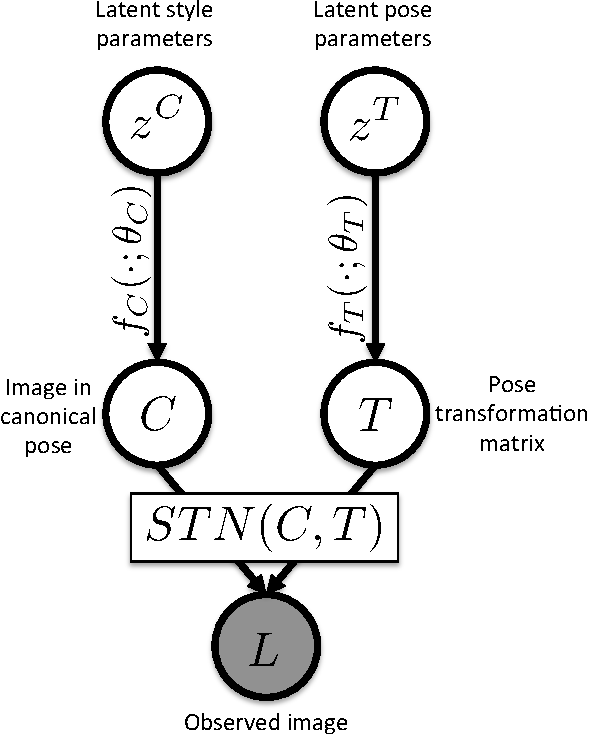
\includegraphics[width=0.25\linewidth]{figs/stvae_gen.pdf}
\label{fig:stvae_decoder}
}\qquad\qquad
\subfigure[]{
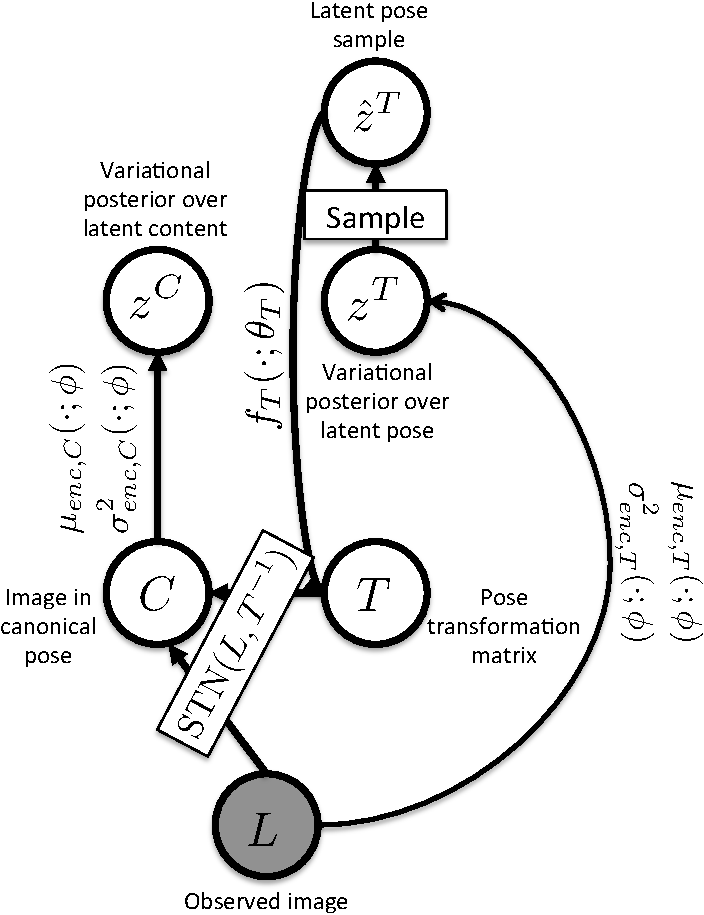
\includegraphics[width=0.3\linewidth]{figs/stvae_rec.pdf}
\label{fig:stvae_encoder}
}\vspace{-5mm}
\end{center}
 \caption{\footnotesize
 \subref{fig:stvae_decoder} ST-VAE Generative model, $P(L | z^C, z^T)$ (Decoder); \subref{fig:stvae_encoder} ST-VAE Recognition model $Q(z^C,z^T | L) = Q(z^C | z^T, L)\cdot Q(z^T | L)$ (Encoder)   
  }\vspace{-5mm}
\label{fig:stvaemodel}
\end{figure}


We focus first on how to parameterize the recognition network (encoder) for the simpler case of a single layer model (i.e., the ST-VAE model
shown in Figure~\ref{fig:stvae_decoder}), in which we need only predict a single set of latent variables $z^C$ and $z^T$.
Na\"{i}vely, one could 
simply use an ordinary MLP to parameterize a distribution $Q(z^C, z^T | L)$, but ideally we would take advantage of the same
 insight that we used for the generative model,
namely 
 that it is easier to recognize content if we separately account for the
 pose.
To this end, we propose the ST-VAE recognition model shown in Figure~\ref{fig:stvae_encoder}. 
Conceptually the ST-VAE recognition model breaks the prediction of $z^C$ and $z^T$ into two stages.  Given the observed image $L$,
we first predict the latent representation of the pose, $z^T$.  Having this latent $z^T$ allows us to recover the pose transformation 
$T$ itself, which we use to ``undo'' the transformation of the generative process
by using the Spatial Transformer Network again but this time with the inverse transformation of the predicted pose.  This result, which can be
thought of as a prediction of the image in a canonical pose, is finally used to predict latent content parameters.


More precisely, we assume that the joint posterior distribution over
pose and content factors as
$Q(z^C, z^T | L) = Q(z^T |L)\cdot Q(z^C | z^T, L)$ where both factors are normal distributions.  
To obtain a draw $(\hat{z}^C, \hat{z}^T)$ from this posterior, we use the following procedure:\vspace{-4mm}

{\footnotesize
\begin{align*}
\hat{z}^T &\sim Q(z^T |L; \phi) = \mathcal{N}(\mu_{T}(L; \phi), \mbox{diag}(\sigma_{T}^2(L; \phi))), \\
\hat{T} &= f_T(\hat{z}^T; \theta_T), \\
\hat{C} &= \mbox{STN}(L, \hat{T}^{-1}), \\
\hat{z}^C &\sim Q(z^C | z^T, L; \phi) =  \mathcal{N}(\mu_{C}(\hat{C}; \phi), \mbox{diag}(\sigma_{C}^2(\hat{C}; \phi))),
\end{align*}\vspace{-4mm}
}

%\kevin{Just write $\mu_{T}()$ instead of $\mu_{enc,T}$. Maybe we need a
%  table summarizing notation?}
where $f_T$ is the pose decoder from the ST-VAE generative model discussed above.
To train an ST-VAE model, we then use the above parameterization of $Q$ and maximize Equation~\ref{eqn:vae_objective} with minibatch
SGD.
As long as the pose and content encoders and decoders  are differentiable, Equation~\ref{eqn:vae_objective} is guaranteed to also be 
end-to-end differentiable.

%To train a model, we
%optimize a similar lower bound as in Equation~\ref{eqn:vae_objective} with respect to parameters of the pose and content encoders/decoders:
%As with the VAE, the ST-VAE objective is fully differentiable end-to-end.




%The Spatially transformed variational auto-encoder is a generative model of images of where pose and content are explicitly separated.  
%We will think specifically of the case where the image is of a single object with a well-defined pose --- though there is nothing about the model
%that prevents it from being applied to arbitrary images.
%Specifically we assume that an image of an object is parameterized by a latent vector of content parameters 
%$z$ as well as a latent vector of pose parameters $\phi$,
%where both $z$ and $\phi$ are drawn independently from distributions $P(z)$ and $P(\phi)$.  
%We then assume that the final observed image is generated by (1) first generating an image $x$ of the object in ``canonical pose'' conditioned on $z$,
%then (2) generating reified transformation parameters $\theta$ conditioned on $\phi$, then (3) transforming the canonical image from the first step to form the 
%final image $x^\theta$.  In our experiments $\theta$ is a vector of entries of a 2d affine transformation matrix, but more general transformations are also possible under our
%framework.  
%By explicitly allowing for  transformations of the image, we make modeling the content a much easier problem since the function $f(z)$ only needs to 
%model the object in a particular canonical pose setting.

%More specifically, the generative ST-VAE model is as follows:
%\begin{align*}
%z,\phi &\sim \mathcal{N}(0, I), \\
%x &= f_z (z), \\
%\theta &= f_\phi (\phi), \\
%x^\theta &= \mbox{STM}(x, \theta),
%\end{align*}
%where $f_z$ and $f_\phi$ are neural networks (MLPs or convolutional networks) which we
%refer to as  the content and pose decoders respectively, following the VAE terminology.
%The function $\mbox{STM}(x, \theta)$ is a \emph{Spatial Transformer Network} module, recently introduced by Jaderberg et al~\cite{jaderberg2015spatial},
%which resamples an image $x$ onto a regular grid which has been transformed by $\theta$ in a fully differentiable manner.
%See Figure~\ref{fig:stvae_decoder} for a graphical representation of the ST-VAE generative distribution.



%We first predict a posterior over latent pose
%$Q(\phi |x^\theta)$.  We then use a sample $\phi\sim Q(\phi | x^\theta)$ and compute transformation parameters $\theta=f_\phi(\phi)$.  We then use
%the Spatial Transformer network again to transform the observed image $x^\theta$, this time using the inverse transformation $\theta^{-1}
%transform the observed image $x^\theta$ 
% which factors
% $Q(z, \phi | x) = Q(z | \phi, x)\cdot Q(\phi|x)$
  
 
 
 


%\subsection{{\bf CST-VAE} Model: Composited Spatially Transformed
 % Variational Auto-encoder}
\subsection{Inference in the CST-VAE model}
\label{sec:cstvae}
\vspace{-3mm}

\begin{figure}[t]
\begin{center}
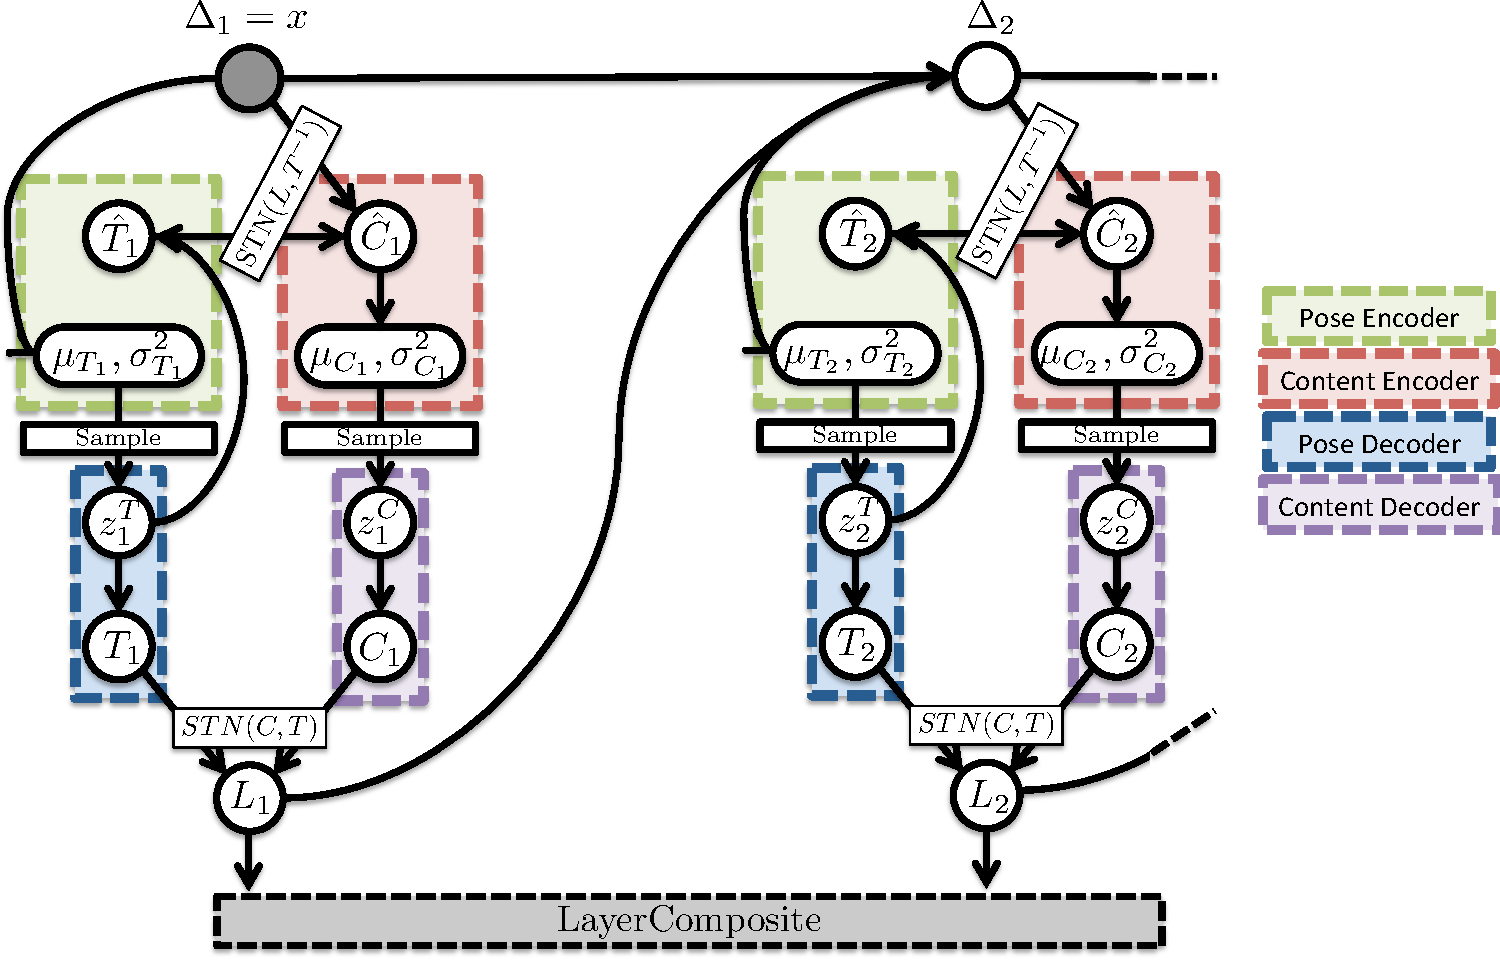
\includegraphics[width=0.65\linewidth]{figs/cstvae_diagram.pdf}\vspace{-4mm}
\end{center}
 \caption{\footnotesize
The CST-VAE network ``unrolled'' for two image layers.
 }\vspace{-4mm}
\label{fig:cstvae}
\end{figure}

%Intuitively the ST-VAE model should work well in factoring pose from content for images of single objects.
%However images generally contain multiple objects of different types with different poses --- we now present
%the Composited Spatially Transformed Variational Auto-encoder  (CST-VAE) model, which is able to factor
%the appearance of an image into the appearance of the different layers
%that create an image.  
%The CST-VAE model thus makes it possible to combine generative models for images
%of single objects to obtain a generative model of  images of multiple objects.  
%Among other things, the CST-VAE model allows us to tease
%apart the component layers (or objects) that make up an image and reason about occlusion.
%Furthermore, as we show in experiments, it can be trained in a fully unsupervised fashion using ordinary stochastic
%gradient descent methods.  %However we can also add labels or use semi supervised methods a la asdfasdf

%In the CST-VAE model, we  assume that images are generated by first independently generating a sequence of layers 
% via the ST-VAE model, then compositing layers from front to back to form a final observed image.  See Figure~\ref{fig:compositestvae_gm} for
% a graphical model depiction of the CST-VAE generative model and Figure~\ref{fig:cartoon}
% for a simplified cartoon illustration of the same process.  We assume that each layer is generated using the same ST-VAE model
% (i.e. parameters are shared across image layers). To composite these layers,  we use  the
%classic \emph{over operator} from computer graphics~\citep{porter1984compositing}.
%In the two-layer setting
%with only foreground and background layers, this over operator reduces to a simple $\alpha$-weighted
%convex combination of foreground and background pixels, but it extends in a natural (and differentiable)
%way to handle multiple layers. % associativity of the over operator

We now turn back to the multi-layer CST-VAE model, where again the task is to parameterize the recognition model $Q$. 
In particular we would like to 
avoid learning a model that must make a ``straight-shot'' joint prediction of all objects and their poses in an image.
Instead our approach is to perform inference over a single layer at a time from front to back, each time removing the contribution of a layer
from consideration until the last layer has been explained.


We proceed recursively: to perform inference for  layer $L_i$, we assume that the latent parameters $z^C_i$ and $z^T_i$ are responsible for explaining
some part of the residual image $\Delta_i$ --- i.e. the part of image that has not been explained by layers $L_1, \dots, L_{i-1}$ (note that $\Delta_1=x$).
We then use the ST-VAE module (both the decoder and encoder modules) 
to generate a reconstruction of the layer $L_i$ given the current residual image $\Delta_i$.  Finally to compute the next residual image to be explained by future layers, we set
$\Delta_{i+1} = \max (0, \Delta_i - L_i)$.  
We use 
the ReLU transfer function, $ReLU(\cdot)=\max(0, \cdot)$,  to ensure
that the residual image can always itself be interpreted as an image
(since 
$\Delta_i-L_i$ can be negative, which breaks interpretability of the
layers).

Note that our encoder for layer $L_i$ requires that the decoder has been run for layer $L_{i-1}$.  Thus it's not possible to separate the generative
and recognition models into disjoint parts as in the ST-VAE model.  Figure~\ref{fig:cstvae} unrolls the entire CST-VAE network (combining
both generative and recognition models) for two layers.
\vspace{-3mm}














